\chapter{Evaluation and Testing}

The system was evaluated as an evidence-collection workflow, not as a simple
classifier. A run is useful only when it reaches a reviewable state: the page
is classified, the right page path is followed, playback or embedded evidence
is inspected, stream or media candidates are collected when available, and
screenshots or traces explain the outcome.

\section{Evaluation Context}

\subsection{Evaluation Objective}

The objective was to measure whether the architecture produced reviewable
evidence and traceable failures. A completed run was not automatically counted
as useful.

\subsection{Website Batch}

The main test object was a regression batch of more than 200 streaming
websites. The batch mixed landing pages, hosting pages, embedded players,
redirects, popup-heavy pages, tokenized streams, and several language/layout
families. The same batch was rerun after prompt, tool, and model changes so
improvements could be compared against previously working sites.

\subsection{Snapshot-Based Evaluation}

The report separates controlled regression-batch metrics from live dashboard
snapshots. Dashboard values describe persisted runs and telemetry at the time
the report was checked. Regression metrics describe selected evaluation runs
and manual acceptance rules. The two views should not be mixed blindly.

\subsection{Manual Review Boundary}

Human review remained part of the evaluation. Screenshots, traces, stream rows,
provider rows, and email drafts were checked to confirm whether a run produced
usable evidence or only a misleading status.

\begin{figure}[!htbp]
\centering
\resizebox{0.96\textwidth}{!}{%
\begin{tikzpicture}[
  protocol/.style={draw=accent!75, fill=blue!4, rounded corners=4pt,
    minimum width=3.25cm, minimum height=1.1cm, text width=2.95cm,
    align=center, font=\small\bfseries},
  review/.style={draw=orange!75!black, fill=orange!10, rounded corners=4pt,
    minimum width=3.2cm, minimum height=1.1cm, text width=2.9cm,
    align=center, font=\small\bfseries},
  telemetry/.style={draw=purple!65!black, fill=purple!7, rounded corners=4pt,
    minimum width=4.2cm, minimum height=1.1cm, text width=3.85cm,
    align=center, font=\small\bfseries},
  compare/.style={draw=green!55!black, fill=green!8, rounded corners=4pt,
    minimum width=3.45cm, minimum height=1.1cm, text width=3.1cm,
    align=center, font=\small\bfseries},
  arr/.style={->, >=Stealth, thick, accent!82, shorten <=3pt, shorten >=3pt},
  ret/.style={->, >=Stealth, thick, gray!65, dashed, shorten <=3pt, shorten >=3pt},
  lab/.style={font=\scriptsize\bfseries, fill=white, inner sep=1.4pt, text=gray!70}
]

\node[protocol] (dataset) at (0,2.35) {Website\\regression batch};
\node[protocol] (execution) at (4.15,2.35) {Pipeline run\\per URL};
\node[protocol] (evidence) at (8.3,2.35) {Evidence\\bundle};
\node[review] (rule) at (12.45,2.35) {Acceptance\\rule};
\node[telemetry] (telemetry) at (4.15,0.25) {Tool, model, and\\cost telemetry};
\node[compare] (compare) at (8.3,0.25) {Regression\\comparison};

\draw[arr] (dataset) -- (execution);
\draw[arr] (execution) -- (evidence);
\draw[arr] (evidence) -- (rule);
\draw[arr] (execution.south) -- (telemetry.north);
\draw[arr] (telemetry) -- (compare);
\draw[arr] (rule.south) |- (compare.east);
\draw[ret] (compare.west) -- ++(-6.0,0) |- node[lab, near start, below]{accept or revise} (dataset.south);

\end{tikzpicture}
}
\caption{Evaluation protocol used for website-batch regression testing.}
\label{fig:evaluation-protocol}
\end{figure}


\begin{table}[!htbp]
\centering
\begin{tabularx}{\textwidth}{Q{4.0cm}Y}
\toprule
\rowcolor{accent!8}
Evaluation item & Value used in the report \\
\midrule
Evaluation snapshot & May 2026 report snapshot. \\
Dataset size & More than 200 streaming websites, selected to cover different
page families and runtime obstacles. \\
Execution unit & One pipeline run per target URL, with classification,
specialist routing, browser-tool execution, evidence capture, and persistence. \\
Main runtime model & \texttt{google\_genai::gemini-3.1-flash-lite}. \\
Prompt/evaluation version & Final regression prompt version after five
prompt/tool iterations. \\
Acceptance rule & A website is counted as working only when the run produces
reviewable evidence, not merely a completed status. \\
Metric sources & Batch results, operator-console telemetry, persisted
tool/model rows, provider-enrichment rows, screenshots, and manual spot checks. \\
Review type & Batch-derived for success rates, dashboard-derived for cost/tool
telemetry, and manual for representative evidence validation. \\
\bottomrule
\end{tabularx}
\caption{Evaluation context for the website regression batch.}
\label{tab:evaluation-context}
\end{table}

\begin{table}[!htbp]
\centering
\begin{tabularx}{\textwidth}{Q{3.6cm}Y Y}
\toprule
\rowcolor{accent!8}
Metric family & Snapshot values & How it should be read \\
\midrule
Run history & 149 total runs, 25 strict successes, 8 partials, 6
\texttt{no\_streams}, 14 \texttt{no\_hosting\_pages}. & Persisted operational
history, not the controlled regression success table. \\
Stream yield & 136 streams, 67 emails, 17.24\% strict stream success. & Live
dashboard evidence yield across persisted terminal runs. \\
Model usage & 83,523,896 total tokens, 1,988 LLM calls, \$15.950543 total
recorded spend. & Dashboard aggregate of model usage rows. \\
Cache visibility & 54,252,590 cached input tokens shown by the dashboard
headline. & Useful for cost analysis, but not forced into the same denominator
as every model breakdown row. \\
Tool telemetry & 3,113 observed tool calls, 3,066 successful calls, 47 failed
calls, 98.49\% observed tool success. & Runtime health indicator for browser
and memory tools. \\
Persistence health & 697 agent runs, 18,094 runtime events, 1,947 persisted
LLM calls, and 3,113 tool calls. & Evidence that the review surface is backed
by normalized records. \\
\bottomrule
\end{tabularx}
\caption{Dashboard snapshot used as operational telemetry, separate from regression-batch metrics.}
\label{tab:dashboard-snapshot}
\end{table}

\section{Evaluation Protocol}

\subsection{Test Input Preparation}

Targets were prepared as website-level URLs rather than isolated media URLs.
This forced the system to handle classification, routing, browser actions, and
evidence capture.

\subsection{Run Execution}

Each run started with classification and then followed the orchestrator route
to landing, hosting, embedded, or terminal status. Browser tools produced
logged outputs and screenshots during the run.

\subsection{Evidence Review}

Evidence was reviewed through screenshots, stream candidates, embedded URLs,
provider/channel context, tool calls, model calls, and final status.

\subsection{Metric Collection}

Metrics came from persisted run rows, dashboard aggregates, tool/model
telemetry, provider records, screenshots, and manual review notes.

\subsection{Regression Comparison}

Changes were accepted only when they improved difficult cases without breaking
previously working ones.

\subsection{Acceptance Rule}

A run is successful only when it gives a reviewer enough evidence and trace
context to understand what happened. A completed status without evidence is not
enough.

\section{Success Metrics}

\begin{table}[!htbp]
\centering
\begin{tabularx}{\textwidth}{Q{4.1cm}Y}
\toprule
\rowcolor{accent!8}
Metric & Definition used during evaluation \\
\midrule
Page classification accuracy & Percentage of URLs routed to the correct page
type: landing, hosting, embedded, blocked, or other. \\
Landing candidate discovery & Share of expected host candidates discovered on
landing pages. \\
Hosting interaction success & Share of hosting attempts where the player state
changed or a meaningful blocker was recorded. \\
Embedded player inspection success & Share of embedded contexts where player
state, stream evidence, or a clear failure reason was captured. \\
Channel detection coverage & Share of accepted evidence runs with visible or
metadata-derived broadcaster/channel context. \\
Stream yield & Share of runs returning a useful manifest, media, iframe,
network, or embedded URL candidate. \\
Strict stream success & Share of runs satisfying the full reviewable stream
evidence rule. \\
Screenshot coverage & Share of runs with meaningful evidence or failure
screenshots. \\
Provider coverage & Share of checked stream or host URLs enriched with
provider or network information. \\
Tool success rate & Successful browser/tool calls divided by total observed
browser/tool calls. \\
Cost per run & Estimated model spend divided by runs in the selected view. \\
\bottomrule
\end{tabularx}
\caption{Success metrics used for agent, tool, provider, and cost evaluation.}
\label{tab:evaluation-metrics}
\end{table}

\section{Agent Regression Results}

\subsection{Baseline Behavior}

Early runs were too broad. Agents sometimes stopped after the first visible
links, harvested before playback, accepted weak screenshots, or continued from
an advertising popup after a click.

\subsection{Prompt and Tool Iterations}

The strongest improvement came from changing the agents from broad
intent-based instructions to a controlled observe--act--verify loop.

\begin{table}[!htbp]
\centering
\begin{tabularx}{\textwidth}{Q{1.4cm}Y Y C}
\toprule
\rowcolor{accent!8}
Version & Main change tested & Regression focus & Working sites \\
\midrule
v1 & Intent-based prompt. & Early stop, weak tab navigation, and premature
harvest. & 38\% \\
v2 & Observe--act--verify loop with explicit tab checks. & Navigation recall
and screenshot-grounded decisions. & 68\% \\
v3 & Popup handling and JavaScript click fallback. & Server activation after
ad traps. & 74\% \\
v4 & Mandatory media-state check before harvest. & Player activation and
stream evidence timing. & 81\% \\
v5 & Tool-budget cap and early success exit. & Cost reduction without losing
previously working websites. & 83\% \\
\bottomrule
\end{tabularx}
\caption{Prompt regression history measured on the website batch.}
\label{tab:prompt-regression}
\end{table}

\subsection{Regression Batch Results}

\begin{table}[!htbp]
\centering
\begin{tabularx}{\textwidth}{Q{4.4cm}C C C}
\toprule
\rowcolor{accent!8}
Metric & Intent v1 & Loop v2 & Current \\
\midrule
Page-type routing accuracy & 91\% & 93\% & 95\% \\
Host-candidate recall & 40\% & 85\% & 89\% \\
Player activation success & 0\% & 70\% & 90\% \\
Popup-interference recovery & 20\% & 55\% & 78\% \\
Tokenized-stream recovery & 25\% & 40\% & 85\% \\
Manifest recovery on AlbaPlayer case & 0\% & 70\% & 90\% \\
Manifest recovery on tokenized Clappr case & -- & 40\% & 85\% \\
\bottomrule
\end{tabularx}
\caption{Main browser-agent KPIs after prompt and tool iterations.}
\label{tab:manual-reference-results}
\end{table}

\begin{figure}[!htbp]
\centering
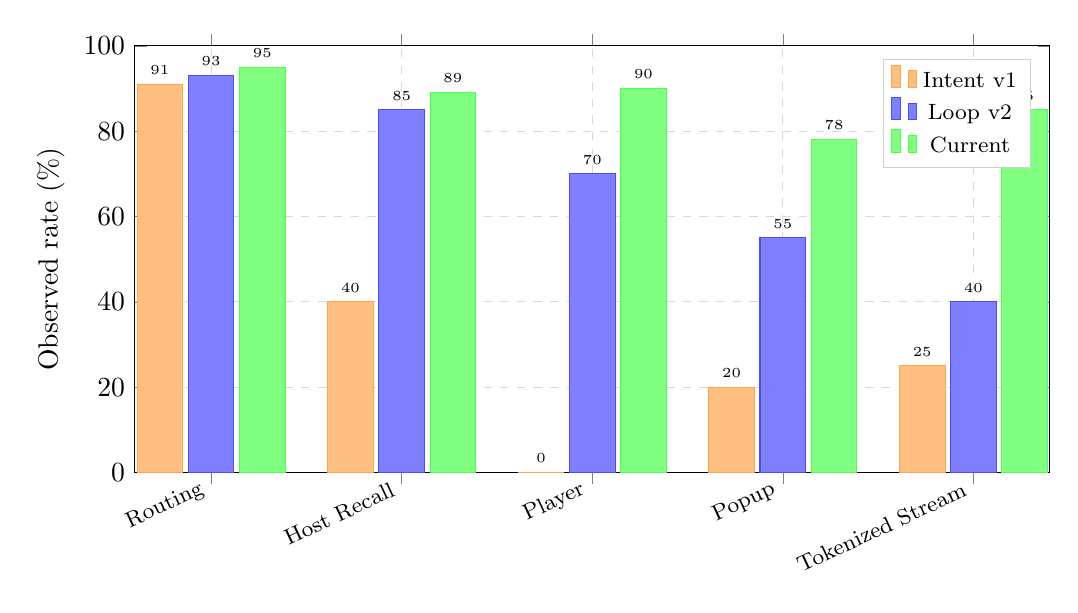
\begin{tikzpicture}
\begin{axis}[
  ybar,
  bar width=0.58cm,
  width=13.2cm, height=7.0cm,
  symbolic x coords={Routing, Host Recall, Player, Popup, Tokenized Stream},
  xtick=data,
  x tick label style={rotate=25, anchor=east, font=\footnotesize},
  ymin=0, ymax=100,
  ylabel={Observed rate (\%)},
  legend style={at={(0.98,0.97)}, anchor=north east, font=\footnotesize, draw=gray!35, fill=white},
  nodes near coords,
  every node near coord/.append style={font=\tiny},
  grid=major, grid style={dashed, gray!30}
]
\addplot[fill=orange!50, draw=orange!70] coordinates {
  (Routing,91)(Host Recall,40)(Player,0)(Popup,20)(Tokenized Stream,25)
};
\addplot[fill=blue!50, draw=blue!70] coordinates {
  (Routing,93)(Host Recall,85)(Player,70)(Popup,55)(Tokenized Stream,40)
};
\addplot[fill=green!50, draw=green!70] coordinates {
  (Routing,95)(Host Recall,89)(Player,90)(Popup,78)(Tokenized Stream,85)
};
\legend{Intent v1, Loop v2, Current}
\end{axis}
\end{tikzpicture}
\caption{Regression-batch improvement across the main browser-agent KPIs.}
\label{fig:manual-kpi-bars}
\end{figure}


\subsection{Improvement Across KPIs}

The results show why evaluation had to be website-level. A classifier can look
accurate while the full investigation fails because the landing agent misses
host candidates or the hosting agent harvests too early.

\subsection{Remaining Agent Failures}

Remaining failures came from anti-bot changes, deep iframe chains, popup-heavy
sites, expired tokenized URLs, incomplete provider metadata, and pages with
mixed landing/hosting signals.

\section{Tool Evaluation}

Tool evaluation checked whether tools were called at the right time, not only
whether they returned a successful status. A browser tool can technically
succeed and still hurt the run if it is used too early, on the wrong tab, or
without follow-up verification. The final evaluation therefore reads tool rows
as an ordered diagnostic trace.

\begin{figure}[!htbp]
\centering
\resizebox{\textwidth}{!}{%
\begin{tikzpicture}[
  node distance=0.9cm,
  symptom/.style={draw=red!65!black, fill=red!5, rounded corners=4pt,
    minimum width=3.55cm, minimum height=0.88cm, align=center, font=\footnotesize\bfseries},
  inspect/.style={draw=accent!75, fill=blue!5, rounded corners=4pt,
    minimum width=3.75cm, minimum height=0.88cm, align=center, font=\footnotesize},
  fix/.style={draw=green!45!black, fill=green!6, rounded corners=4pt,
    minimum width=3.75cm, minimum height=0.88cm, align=center, font=\footnotesize},
  arrow/.style={->, >=Stealth, thick, gray!75}
]

\node[symptom] (s1) {No hosting candidates};
\node[symptom, below=0.38cm of s1] (s2) {Player not activated};
\node[symptom, below=0.38cm of s2] (s3) {No stream after harvest};
\node[symptom, below=0.38cm of s3] (s4) {Wrong page or popup};
\node[symptom, below=0.38cm of s4] (s5) {Provider contact missing};

\node[inspect, right=1.15cm of s1] (i1) {Landing inspect output\\candidate ledger, screenshots};
\node[inspect, below=0.38cm of i1] (i2) {Hosting trace\\click result, media state};
\node[inspect, below=0.38cm of i2] (i3) {Harvest diagnostics\\network, iframe, video state};
\node[inspect, below=0.38cm of i3] (i4) {Tab and frame events\\final URL, active page};
\node[inspect, below=0.38cm of i4] (i5) {Provider rows\\host, IP, lookup status};

\node[fix, right=1.15cm of i1] (f1) {Reveal sections\\rank candidates};
\node[fix, below=0.38cm of f1] (f2) {Try server controls\\verify after action};
\node[fix, below=0.38cm of f2] (f3) {Delay harvest\\require readiness};
\node[fix, below=0.38cm of f3] (f4) {Close popup\\restore focus};
\node[fix, below=0.38cm of f4] (f5) {Keep partial context\\flag missing contact};

\draw[arrow] (s1) -- (i1);
\draw[arrow] (s2) -- (i2);
\draw[arrow] (s3) -- (i3);
\draw[arrow] (s4) -- (i4);
\draw[arrow] (s5) -- (i5);
\draw[arrow] (i1) -- (f1);
\draw[arrow] (i2) -- (f2);
\draw[arrow] (i3) -- (f3);
\draw[arrow] (i4) -- (f4);
\draw[arrow] (i5) -- (f5);

\node[font=\small\bfseries\color{accent}, above=0.35cm of s1] {Failure symptom};
\node[font=\small\bfseries\color{accent}, above=0.35cm of i1] {Records to inspect};
\node[font=\small\bfseries\color{accent}, above=0.35cm of f1] {Engineering response};

\end{tikzpicture}%
}
\caption{Failure-diagnostics map used during evaluation: each visible failure is traced to specific records and a concrete engineering response.}
\label{fig:failure-diagnostics-map}
\end{figure}


\subsection{Navigation Tools}

Navigation was evaluated by whether it reached the intended page, returned the
final URL/status, handled challenge timing, and preserved screenshots. The
important failure was not simple navigation failure. It was navigation at the
wrong moment: leaving a page after the player had already been activated,
resetting server state, or treating a same-page tab as a full URL transition.
The corrected policy uses navigation for URL changes and interaction tools for
player controls, tabs, and buttons.

\subsection{Inspection Tools}

Inspection was evaluated by whether it exposed the page role, candidate links,
element handles, frame paths, playback state, and profile-specific evidence
without excessive output. Broad inspection is useful after navigation or after
a meaningful state change, but repeated broad reads waste context and can hide
the next concrete action. The final policy is to inspect broadly once, then use
targeted element detail, frame detail, or media-state tools for local decisions.
Profile-specific inspection was especially important: landing pages need
candidate discovery, hosting pages need server/player state, and embedded pages
need player-focused evidence.

\subsection{Interaction Tools}

Interaction was evaluated by whether clicks, plays, typing, selections, and
coordinate actions changed the intended page state and were followed by
verification. The main observed failures were popup focus loss, wrong-control
clicks, hidden server buttons, and actions accepted without checking page
state. The final prompt and tool policy require verification after interaction:
a screenshot, media-state check, focused inspect result, or stream harvest
after readiness. This changed interaction from blind clicking into a measured
observe--act--verify step.

\subsection{Evidence Capture and Harvesting Tools}

Evidence tools were evaluated by whether screenshots captured meaningful
states and whether stream harvesting happened after playback or player
readiness. Early runs often harvested before the player generated network
requests, which produced false \texttt{no\_streams} results. The final policy
uses screenshot checkpoints, media-state checks, delayed harvest, and iframe
diagnostics before declaring failure. Stream evidence is only useful when it is
connected to the page, frame, timestamp, and visible state that produced it.

\subsection{Tool Modes and Output-Size Tradeoffs}

The final tool policy prefers one broad inspect after navigation or meaningful
state change, then targeted detail tools for the next action. This reduced
repeated broad context and made tool output easier for agents to use.

This tradeoff is important because browser pages can produce very large DOM
summaries. Large outputs increase model cost and can distract the agent from
the useful next action. The final tool design separates compact page context,
targeted element reads, profile-specific inspection, screenshots, and harvest
diagnostics so the agent can ask for the smallest useful evidence.

\subsection{Tool Regression Fixes}

\begin{table}[!htbp]
\centering
\begin{tabularx}{\textwidth}{Q{2.7cm} Y Y Y Y}
\toprule
\rowcolor{accent!8}
Tool category & Expected behavior & Main failures & Fixes & Evaluation signal \\
\midrule
Navigation & Reach intended URL or state and return final URL/status. &
Challenge pages, redirects, overshot pages. & Challenge wait/retry, final URL
recording, screenshots. & Correct route state and traceable blocked pages. \\
Inspection & Produce usable page, element, frame, and media state. & Repeated
broad reads, missing hidden sections, weak frame context. & Profile inspect
tools, targeted detail reads, frame paths. & Better candidate discovery and
lower context waste. \\
Interaction & Change the intended page state. & Popup focus loss, wrong tab,
premature server switching. & Popup close, focus restore, locator strategies,
verify-after-action. & Player activation and popup recovery improved. \\
Evidence capture and harvesting & Preserve screenshots and media evidence after
state readiness. & Screenshots before activation, harvest before media
requests. & Media-state guard, delayed harvest, screenshot checkpoints. &
Higher stream and manifest recovery. \\
Memory support & Provide reusable hints without replacing live evidence. &
Stale selectors or overconfident remembered paths. & Treat memory as hint,
update only after live confirmation. & Fewer repeated dead-end explorations. \\
\bottomrule
\end{tabularx}
\caption{Tool evaluation by category.}
\label{tab:tool-evaluation-by-category}
\end{table}

\begin{table}[!htbp]
\centering
\begin{tabularx}{\textwidth}{Q{3.6cm}Y Z{3.0cm}}
\toprule
\rowcolor{accent!8}
Tool finding & Evaluation meaning & Observed value / fix \\
\midrule
Observed tool calls & Browser/tool invocations with persisted outcome rows. &
3,113 \\
Successful calls & Calls that returned a successful tool outcome. & 3,066 \\
Failed calls & Calls that returned an error or failed outcome. & 47 \\
Tool success rate & Successful observed calls divided by observed tool calls. &
98.49\% \\
Average duration & Mean observed duration per tool call. & 7.636 s \\
Calls per run & Approximate observed browser/tool actions per persisted run. &
20.9 \\
Premature harvest & \texttt{harvest()} ran before playback produced media
evidence. & Activation guard and media-state check. \\
Wrong tab/focus & Agent reasoned over an advertising tab instead of the player
tab. & Popup close and focus restore. \\
Navigation misuse & Same-page controls were opened with navigation instead of
click interaction. & Clearer \texttt{interact} versus \texttt{navigate}
policy. \\
\bottomrule
\end{tabularx}
\caption{Tool-health telemetry and main tool-regression fixes.}
\label{tab:tool-regression-summary}
\end{table}

\section{Model, Token, Cost, and Cache Behavior}

\subsection{Runtime Model Choice}

The final runtime used \texttt{google\_genai::gemini-3.1-flash-lite}. The
choice was based on operating behavior: long browser traces, predictable tool
use, latency during browser loops, and repeated-batch cost
\cite{gemini-pricing,gemini-caching,gemini-rate-limits,openrouter-models}.

\subsection{Input and Output Token Usage}

\subsection{Cached Input Tokens}

\subsection{Cost per Run}

\begin{table}[!htbp]
\centering
\begin{tabularx}{\textwidth}{Q{4.0cm}Y Z{3.0cm}}
\toprule
\rowcolor{accent!8}
Metric & Interpretation & Observed value \\
\midrule
Selected model & Default model for the final regression snapshot. &
Gemini 3.1 Flash-Lite \\
Total model spend & Sum of recorded or estimated model usage rows in the
dashboard snapshot. & \$15.950543 \\
Average cost per run & Dashboard spend normalized by terminal runs with
recorded usage. & \$0.110004 \\
LLM calls & Model invocations shown by the dashboard aggregate. & 1,988 \\
Input tokens & Prompt, trace, tool-context, and memory tokens recorded by the
dashboard aggregate. & 82,506,629 \\
Cached input tokens & Cached input shown by the dashboard headline card. &
54,252,590 \\
Output tokens & Generated model tokens in the dashboard aggregate. & 1,017,267 \\
Total tokens & Input and output tokens shown by the overview tab. & 83,523,896 \\
\bottomrule
\end{tabularx}
\caption{Model, token, cost, and cache telemetry used during evaluation.}
\label{tab:model-cost-summary}
\end{table}

\subsection{Cost-Control Lessons}

The cost view, cache view, and headline token card may not share exactly the
same denominator when runs have partial usage rows or provider aliases. The
important lesson is the split between input, cached input, output, calls, and
spend, because repeated batches become expensive without prompt and context
reuse.

\section{Provider and Channel Enrichment Evaluation}

\subsection{Channel Detection Results}

Channel detection was evaluated as coverage, not certainty. A run could expose
channel context through visible labels, DOM text, screenshot evidence, stream
metadata, or provider context. Missing channel context remained explicit.

\subsection{Provider Resolution}

Provider analysis runs after stream or embedded URLs are collected. It resolves
hostnames, checks whether routable IP addresses are available, and enriches the
result with provider or registration data through IP and RDAP/WHOIS sources
\cite{ipinfo-api,icann-rdap}.

\subsection{Abuse Contact Availability}

An abuse contact is useful but not required for provider coverage. Some
providers or networks can be identified without exposing a direct contact.

\subsection{CDN and Hosting Context}

Provider context helps reviewers understand where the stream host appears to be
served from, but it does not prove infringement by itself.

\subsection{Enrichment Limitations}

Provider data can be incomplete, stale, masked by CDNs, or missing direct abuse
contacts. These fields remain subject to human review.

\begin{table}[!htbp]
\centering
\begin{tabularx}{\textwidth}{Q{3.8cm}Y Z{2.8cm}}
\toprule
\rowcolor{accent!8}
Provider metric & Meaning & Observed value \\
\midrule
Provider analysis records & Stream or media evidence rows enriched by the
provider stage. & 136 \\
Runs with stream evidence & Runs that produced at least one stream candidate in
the dashboard snapshot. & 25 \\
Total stream records & Persisted stream records shown by the overview tab. &
136 \\
Generated email drafts & Review drafts generated from stream/provider evidence.
& 67 \\
Unique provider names & Distinct provider names shown in the overview
breakdown. & 12 \\
Largest provider group & Most frequent provider in the snapshot. & TECHOFF SRV
LIMITED, 38 analyses \\
\bottomrule
\end{tabularx}
\caption{Provider-enrichment telemetry for extracted stream evidence.}
\label{tab:provider-intelligence-values}
\end{table}

\section{Representative Evaluation Cases}

\subsection{Landing Page With Repeated Event Cards}

Some landing pages list repeated match cards by date, league, or channel. Early
runs collected only visible links. The fix required landing-specific
inspection, checked-section tracking, reveal actions, and candidate ranking.

\subsection{Hosting Page With Popup Interference}

Hosting pages often opened popups after play clicks. The fix required popup
closing, focus restoration, screenshot checkpoints, and safer click strategies.

\subsection{Embedded Player With Delayed Manifest}

Embedded players sometimes emitted manifests only after play activation and a
short wait. The fix required media-state checks and delayed harvest rather than
immediate extraction.

\subsection{Tokenized Stream URL}

Tokenized URLs can expire after the run. The evidence bundle therefore stores
the URL exactly as observed with timestamp, source page, frame context,
screenshot, and provider context.

\subsection{Wrong Page Classification}

Mixed-role pages can contain both listing and player signals. The classifier
therefore considers visible page role, player signals, iframe context, and the
action needed, not only URL shape.

\subsection{Provider or Channel Enrichment Without Complete Contact Data}

Provider or channel context can be useful even when abuse contact or
rights-holder mapping is incomplete. The final evaluation separates provider
coverage, channel detection, and contact availability.

\section{Remaining Limitations}

\subsection{Runtime Instability}

Some sites change JavaScript or anti-bot behavior between runs. A path that
worked during the batch can fail later.

\subsection{Website Volatility}

Selectors, player vendors, mirrors, iframes, and stream hosts change
frequently. Continuous monitoring and regression are still required.

\subsection{Anti-Bot and Blocking Cases}

Challenge pages, rate limits, and blocked browser sessions can stop evidence
collection. The system should record these cases rather than hide them.

\subsection{Incomplete Provider or Channel Metadata}

Provider, channel, and abuse-contact data can be incomplete or unavailable.
Human review remains necessary.

\subsection{Evaluation Scope}

The numbers are a regression snapshot, not a guarantee that every future
streaming site will behave the same way. Larger labeled batches and longer
monitoring would strengthen confidence.

\section{Chapter Summary}

The evaluation supports the internship contribution because it measures the
complete investigation path. The system improved from weak intent-based
behavior to a controlled browser-agent workflow with higher website success,
clearer tool discipline, measurable model cost, cache visibility, and
provider/channel enrichment. Most importantly, the evaluation method gives
future work a practical rule: accept a change only when it adds coverage
without losing evidence that already worked.
